\documentclass[8pt]{beamer}

\usetheme{Darmstadt}
\usecolortheme{dove}
\usepackage[small,center]{caption}
\usepackage{times}
\usefonttheme{structurebold}
\usepackage[english]{babel}
\usepackage{pgf,pgfarrows,pgfnodes,pgfautomata,pgfheaps}
\usepackage{amsmath,amssymb}
\usepackage{amsxtra}

\usepackage{caption}
\usepackage{tikz}
\usetikzlibrary{shapes.misc}

\newcommand{\leftd}[1]{{\color{red} \bar{#1}}}
\newcommand{\interface}[2]{{\color{blue}{#1}_I(#2)}}
\newcommand{\leftdd}[2]{{\color{red} \bar{#1}(\bar{#2})}}
\newcommand{\leftFourier}[1]{{\color{red} \hat{#1}}}
\newcommand{\leftFourierTwo}[2]{{\color{red} \hat{#1}(\hat{#2})}}
\newcommand{\half}{\dfrac{1}{2}}
\newcommand{\divergence}{\mathrm{div}}

\newcommand{\I}{I}

\newcommand*{\vcenterimage}[1]{\vcenter{\hbox{\includegraphics[width=2in]{#1}}}}
\newcommand*{\vcenterarrow}{\vcenter{\hbox{$\Longrightarrow$}}}

\DeclareMathOperator{\hyphen}{-}

\definecolor{Carolinablue}{RGB}{75, 156, 211}
\definecolor{ballblue}{rgb}{0.13, 0.67, 0.8}
\definecolor{lightgray}{rgb}{0.83, 0.83, 0.83}
\setbeamercolor{block title}{bg=lightgray,fg=Carolinablue}
\setbeamercolor{block body}{bg=white,fg=black}
\setbeamercovered{dynamic}
\setbeamercolor*{item}{fg=Carolinablue}

\captionsetup[subfigure]{labelformat=empty}
\captionsetup[figure]{labelformat=empty}
\setbeamertemplate{navigation symbols}{}
\setbeamertemplate{footline}[frame number]
\begin{document}

% tikz stuff
\tikzset{cross/.style={cross out, draw=black, minimum size=2*(#1-\pgflinewidth),
inner sep=0pt, outer sep=0pt},
%default radius will be 1pt.
cross/.default={2.5pt}}



\frame{
\title{\Large Realistic Cardiac Simulations with IBAMR}

\author{{\Large David Wells \\\vspace{0.1in} University of North Carolina}    \\
\vspace{0.2in} {Cardiovascular Modeling and Simulation Lab}}

\date{June 7, 2019\\{}}

\begin{figure}[h]
\centering

\includegraphics[width=1.5in]{UNC_logo_542.eps}
 \end{figure}%

\vspace{-0.2in}
\titlepage
}

\begin{frame}
    \frametitle{Outline}
    Collaborators
    \begin{itemize}
    \item[$\blacksquare$] Charles Puelz (NYU)                                 \\
    \item[$\blacksquare$] Boyce Griffith, Simone Rossi, Margaret-Anne Smith,
    Aaron Barrett (UNC)                                                       \\
    \item[$\blacksquare$] Paul Segars, Greg Sturgeon (Duke)
    \item[$\blacksquare$] Matt Knepley (SUNY Buffalo)                         \\
    \end{itemize}
\end{frame}

\begin{frame}
    \frametitle{Outline}
    Content of this talk:
    \begin{itemize}
    \item[$\blacksquare$] Background                                          \\
    \item[$\blacksquare$] Relevant Equations                                  \\
    \item[$\blacksquare$] Fluid-Structure Interaction                         \\
    \item[$\blacksquare$] The IB Method                                       \\
    \item[$\blacksquare$] Where do we use PETSc?                              \\
    \end{itemize}
\end{frame}

\section{Background}
\begin{frame}
    \frametitle{The Human Heart}
    \begin{figure}
        \centering
        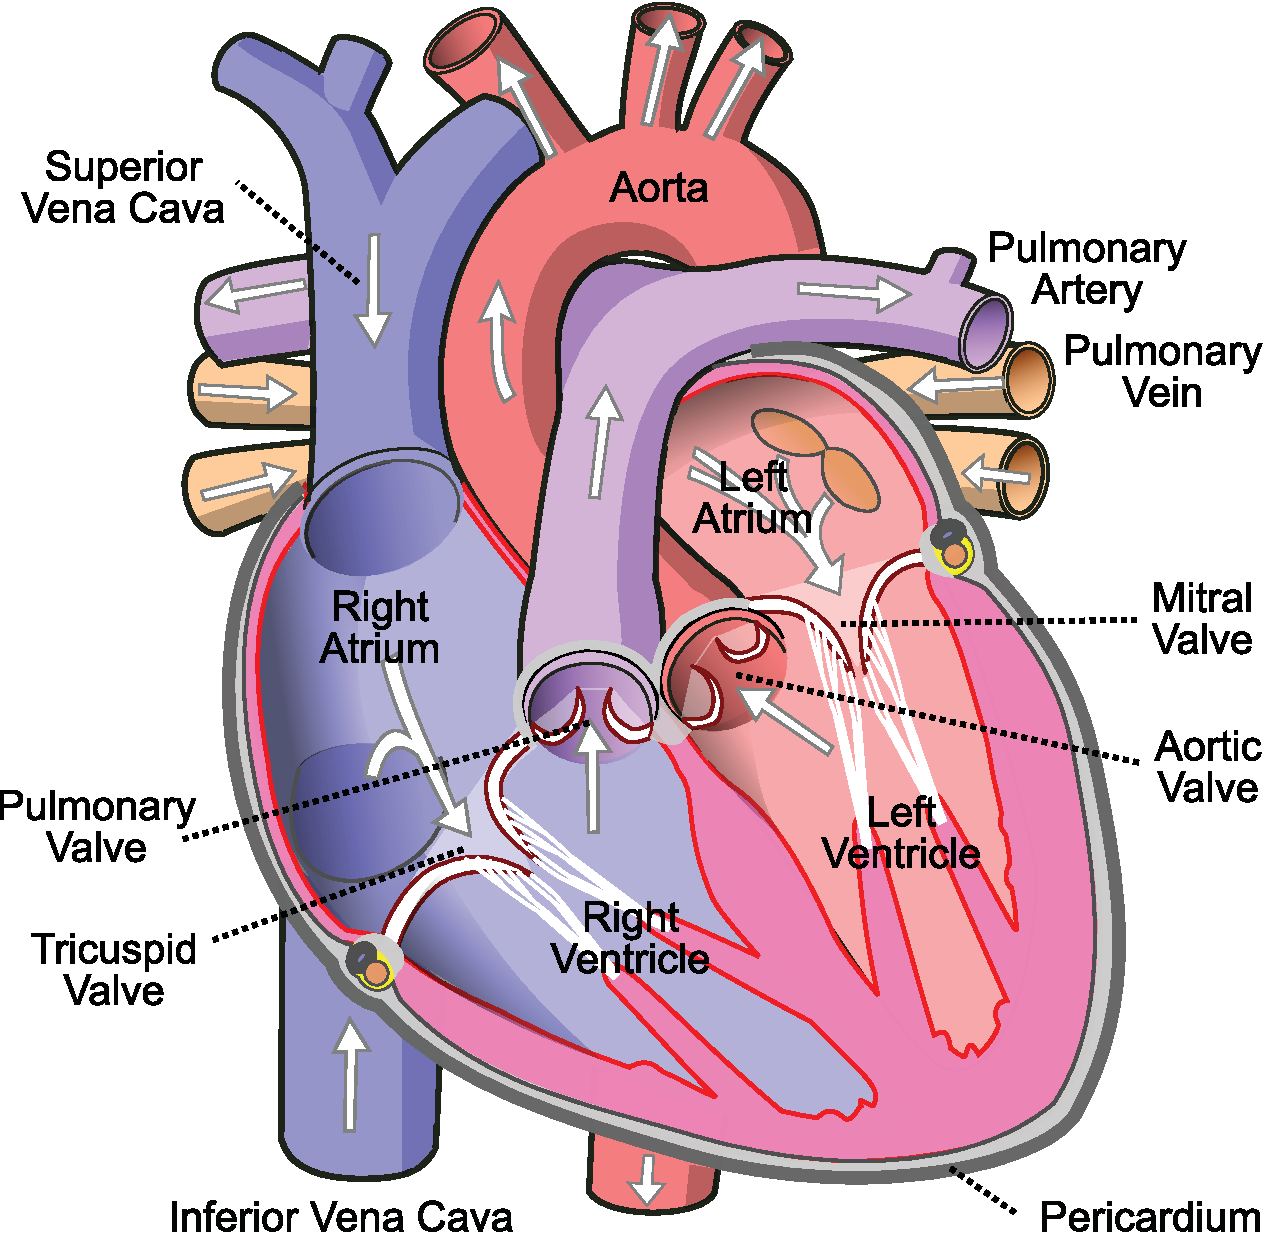
\includegraphics[width=2in]{diagram-of-the-human-heart.pdf}
    \end{figure}
    \begin{itemize}
        \item[$\blacksquare$] 300,000 valve replacement surgeries each year
        \item[$\blacksquare$] Accurate simulations of the cardiac cycle
        \item[$\blacksquare$] Current emphasis: realistic valve dynamics, better
        parallel scaling
    \end{itemize}
\end{frame}

\begin{frame}
    \frametitle{Incompressible Fluids, Hyperelastic Incompressible Structures}
    \begin{figure}
        \centering
        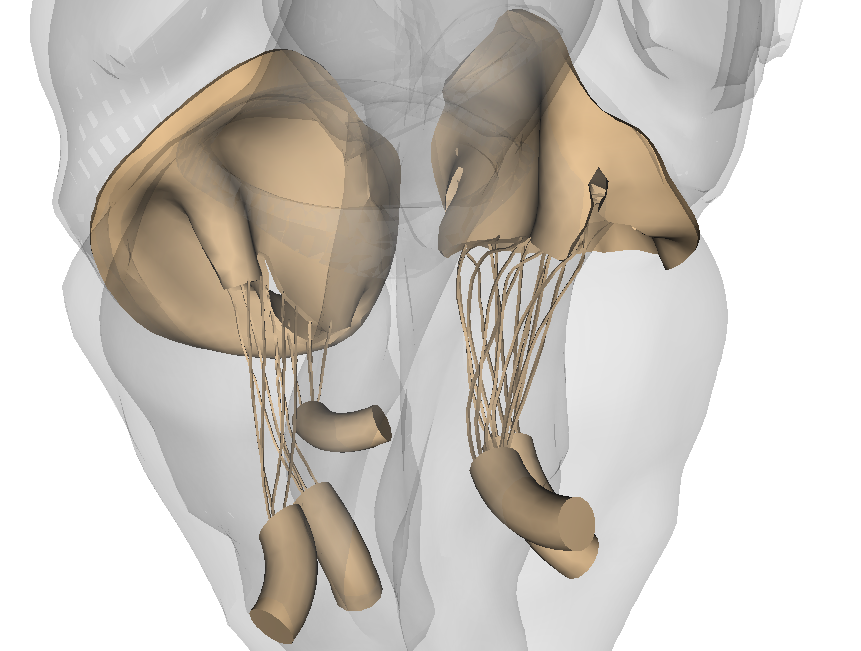
\includegraphics[width=2in]{mv_tv_front0037.png}
    \end{figure}
    \begin{itemize}
        \item[$\blacksquare$] Navier-Stokes: finite differences on a Cartesian grid
        \item[$\blacksquare$] Finite strain elasticity: finite elements on an
        unstructured mesh
        \item[$\blacksquare$] Coupled with the immersed boundary (IB) method
    \end{itemize}
    The fluid and structure are assumed to have equal densities (neutral
    buoyancy).
\end{frame}

\begin{frame}
    \frametitle{Computational Glossary}
    \begin{itemize}
        \item[$\blacksquare$] \emph{IBAMR}: Immersed Boundary Adaptive Mesh
        Refinement (software package at UNC; collaborators at UCSD, SUNY
        Buffalo, NWU, etc.) \texttt{https://www.github.com/IBAMR/IBAMR}
        \item[$\blacksquare$] \emph{Cell}: One cell in the Eulerian grid
        (managed by SAMRAI)
        \item[$\blacksquare$] \emph{Patch/Box}: A collection of Eulerian cells
        (between \(8x8x8\) and \(512x512x512\)) owned by one processor
        \item[$\blacksquare$] \emph{Element}: One element in (managed by
        libMesh) one of the structures
        \item[$\blacksquare$] \emph{Quadrature Point}: Point for numerical
        integration. Points at which we couple the fluid and structure.
    \end{itemize}
\end{frame}

\section{Relevant Equations}
\begin{frame}
    \frametitle{Marker and Cell (MAC) scheme for incompressible flow}
    \begin{figure}
        \centering
        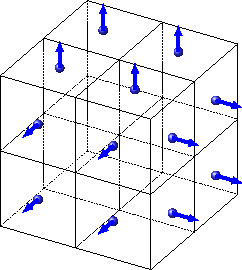
\includegraphics[width=2in]{face-centered.pdf}
    \end{figure}
    \begin{itemize}
        \item[$\blacksquare$] An oldie, but a goodie (LANL 1965)
        \item[$\blacksquare$] Staggered discretization: face-centered
        velocities, cell-centered pressure
        \item[$\blacksquare$] No checkerboard instability
        \item[$\blacksquare$] In practice: much better (10-100x) volume
        conservation than collocated differences
    \end{itemize}
\end{frame}

\begin{frame}
    \frametitle{Marker and Cell (MAC) scheme for incompressible flow}
    \begin{figure}
        \centering
        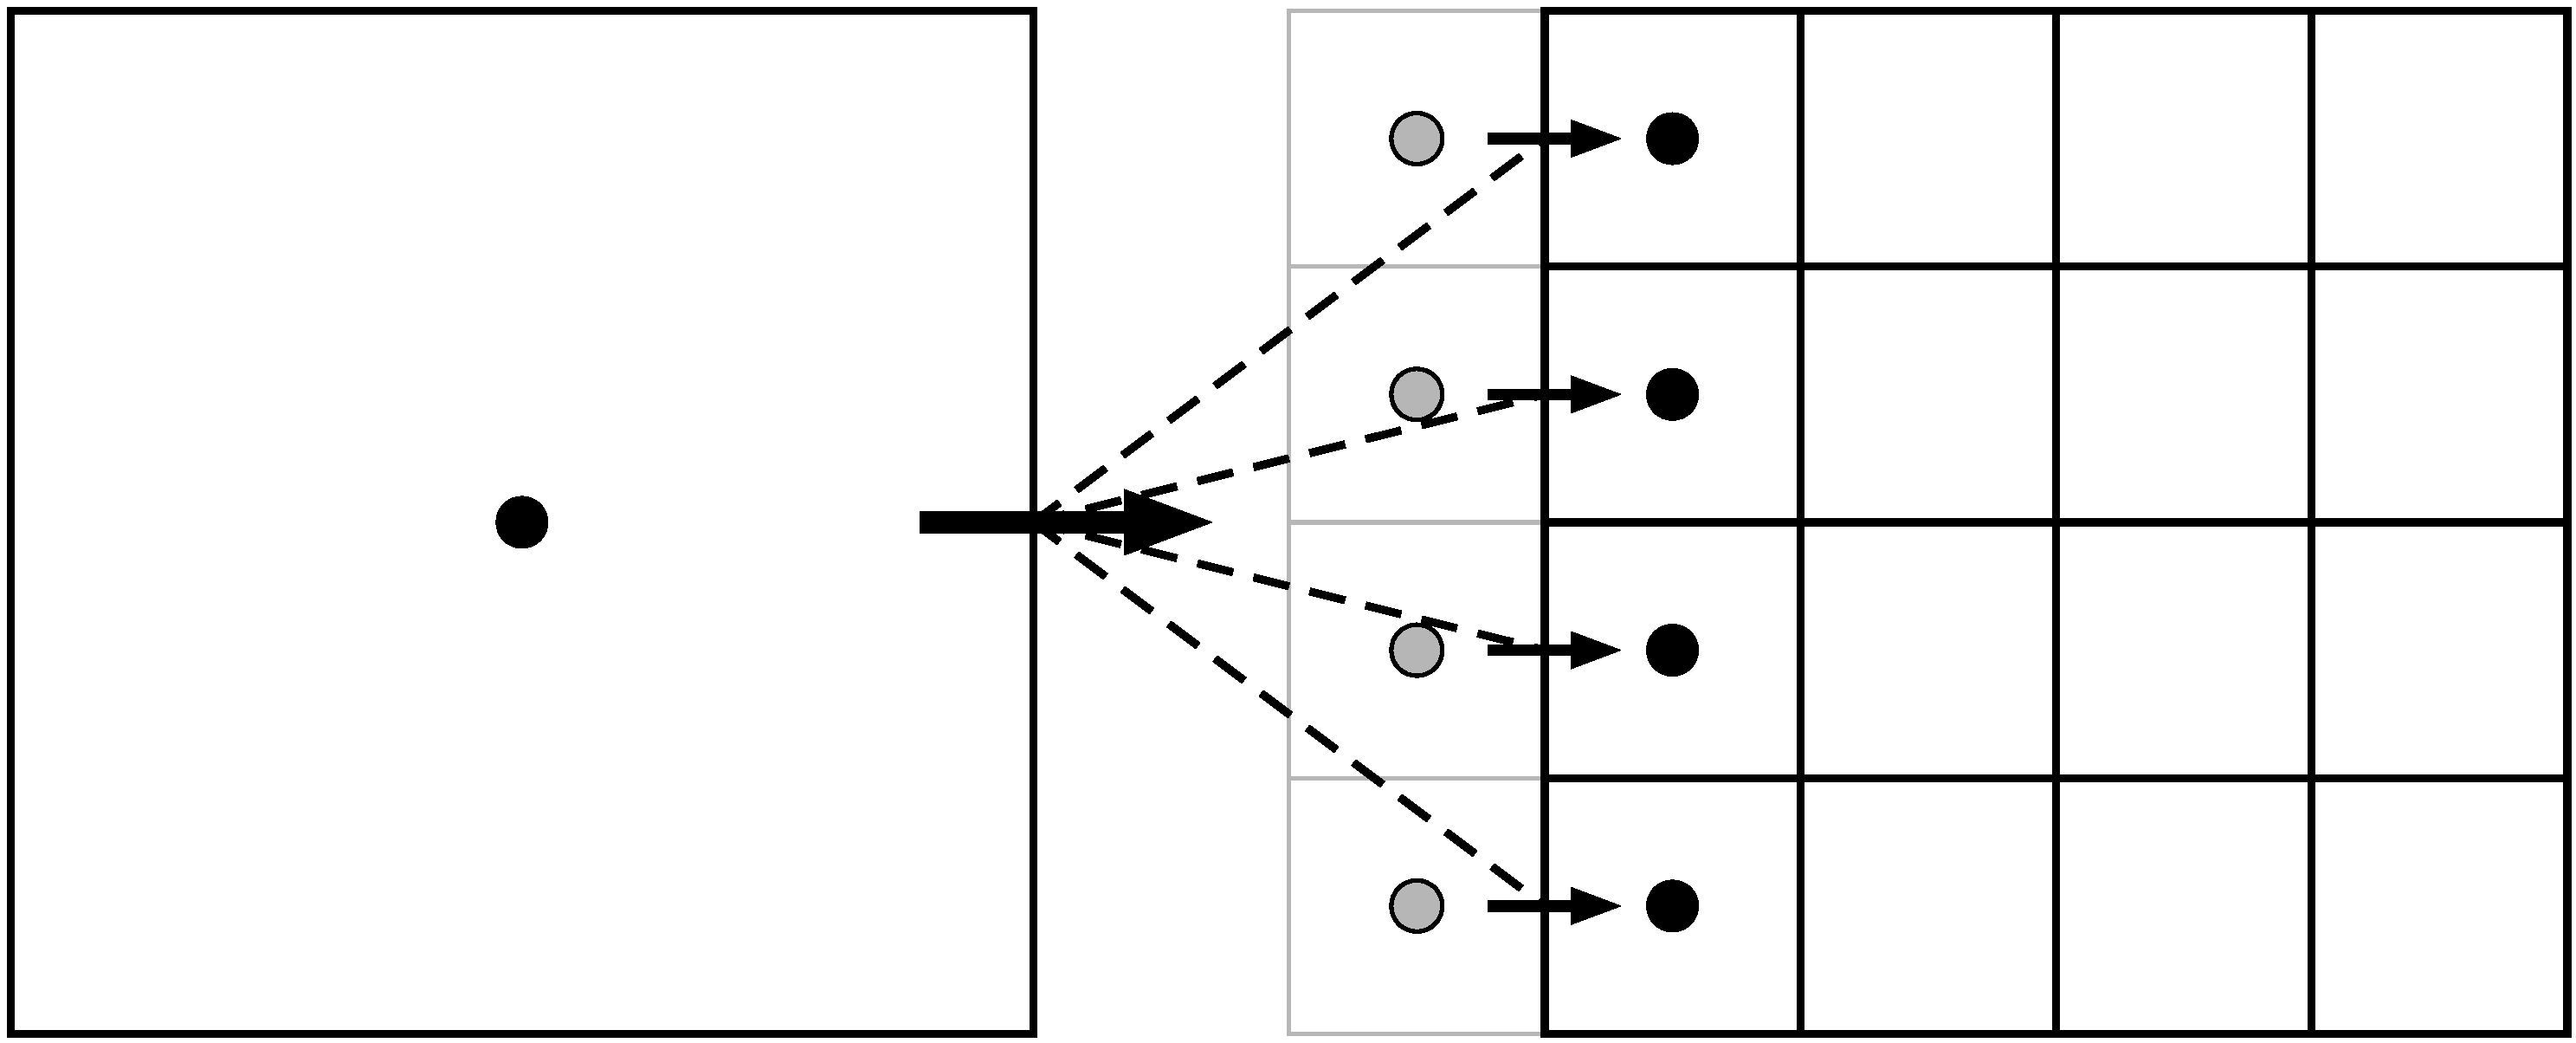
\includegraphics[width=2.5in]{cf_interface_6-1380.pdf}
    \end{figure}
    \begin{itemize}
        \item[$\blacksquare$] Cubic interpolation to compute coarse-to-fine
        ghost values
        \item[$\blacksquare$] Conserves momentum on each cell (Griffith, 2012)
        \item[$\blacksquare$] \emph{work in progress}: SPD Laplacians for
        creeping flow, complex fluids (with Aaron Barrett, Boyce says Toby knows
        how to do this)
    \end{itemize}
\end{frame}

\begin{frame}
    \frametitle{Fluid Discretization with SAMR}
    \begin{figure}
        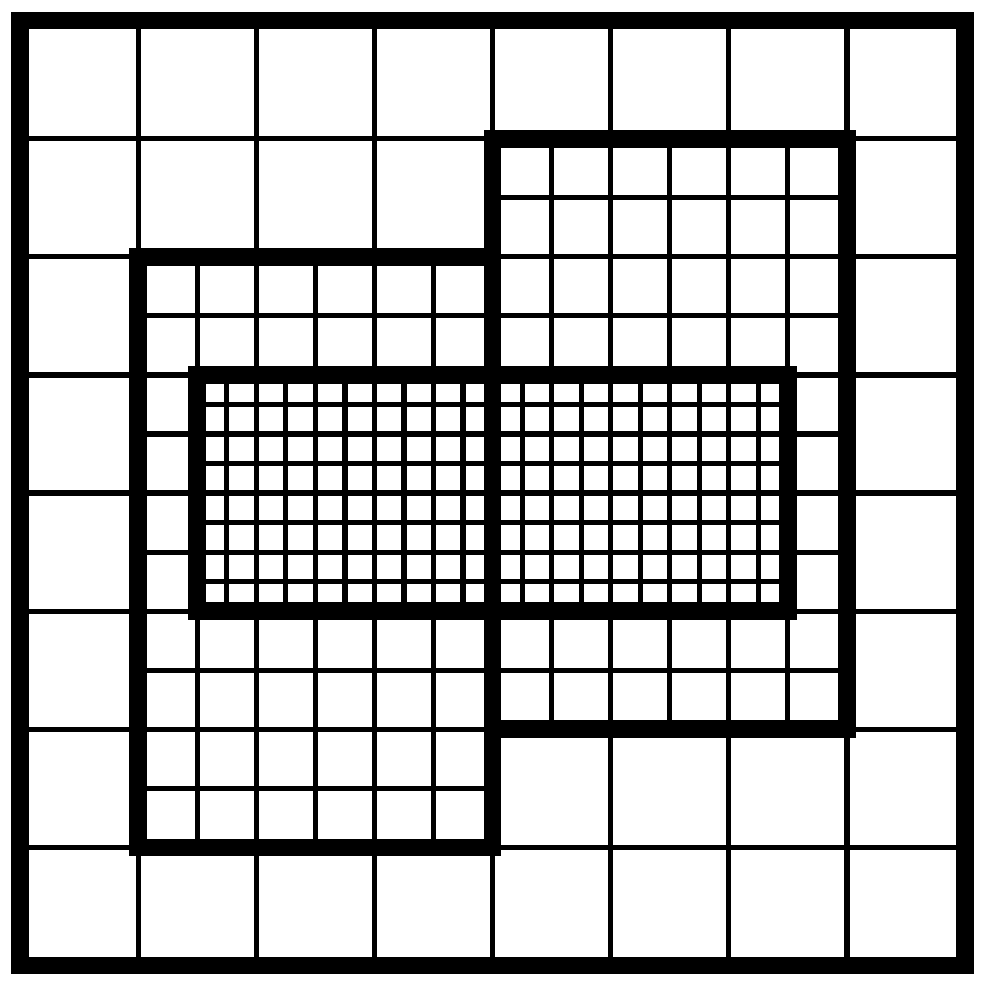
\includegraphics[width=2in]{valid-grid-3-levels.pdf}
    \end{figure}
    \begin{itemize}
        \item[$\blacksquare$] \textbf{S}tructured \textbf{A}daptive \textbf{M}esh \textbf{R}efinement
        \item[$\blacksquare$] Finite differences on Cartesian grids: fast solvers
        \item[$\blacksquare$] Fine cells placed on structures and near important
        flow features
        \item[$\blacksquare$] Boundary conditions: simplified circuit-like
        models of the human body (\emph{ongoing work}), do-nothing BC away from structure
    \end{itemize}
\end{frame}

\begin{frame}
    \frametitle{Fluid Discretization with SAMR}
    \begin{figure}
        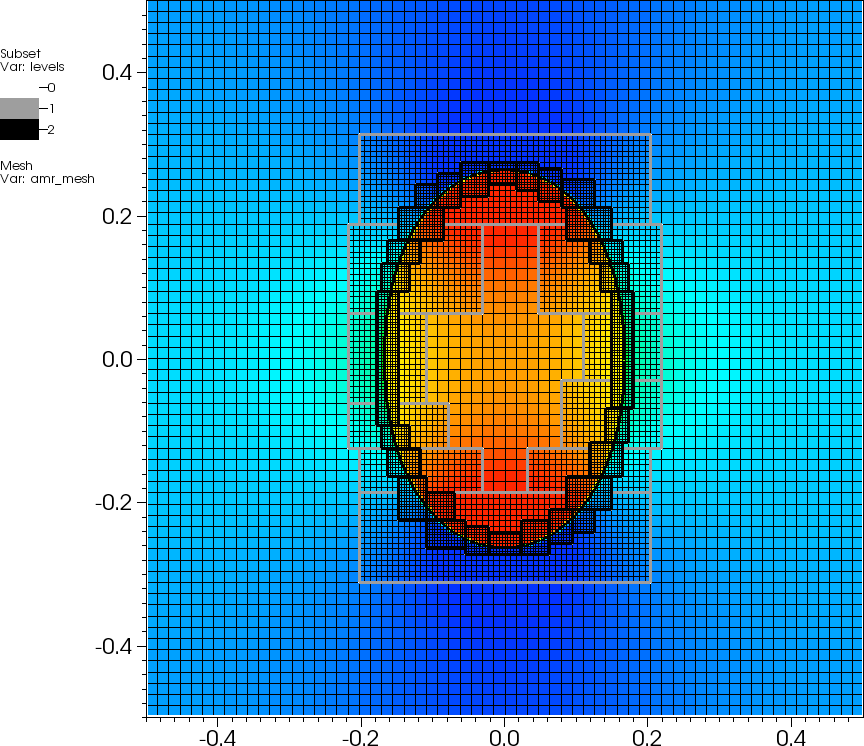
\includegraphics[width=3in]{curve2d_levels_mesh-93-361.png}
    \end{figure}
    \begin{itemize}
        \item[$\blacksquare$] Currently use SAMRAI 2: migrating to SAMRAI 3
    \end{itemize}
\end{frame}

\begin{frame}
    \frametitle{Fiber-reinforced hyperelastic model of the aortic root}
    \begin{figure}
        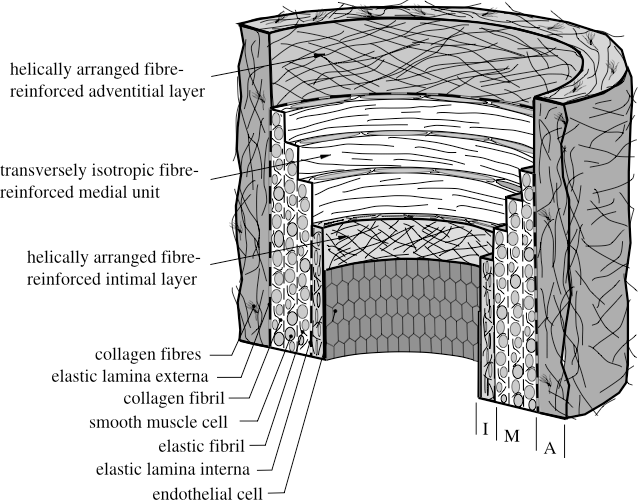
\includegraphics[width=3in]{vessel_schematic-904.png}
    \end{figure}
    A fiber-reinforced hyperelastic constituitive model (Gasser, Ogden,
    Holzapfel, 2006)
\end{frame}

\begin{frame}
    \frametitle{Finite Element Approximation of Elastic Structures}
    \begin{figure}
        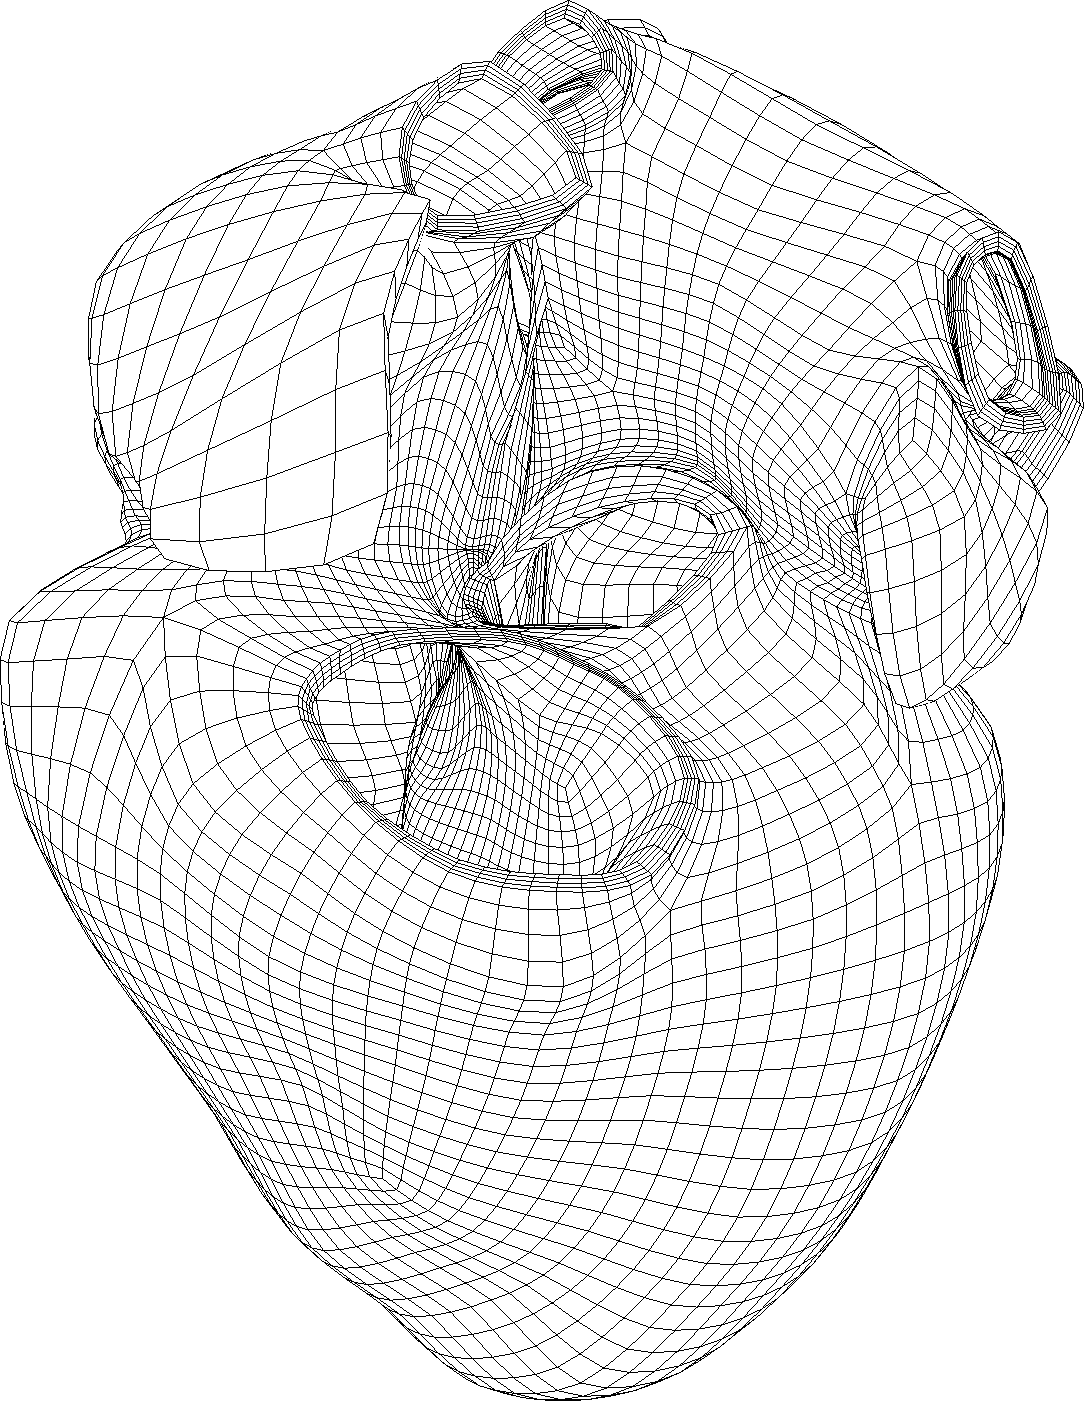
\includegraphics[width=2in]{heartmesh1.png}
    \end{figure}
    The velocity of the structure is completely determined by the velocity of
    the fluid.
\end{frame}

\begin{frame}
    \frametitle{Fiber-reinforced hyperelastic model of the aortic root}
    Here \(\chi(\mathbf{X}, t)\) is the position of the structure and
    \(\mathbf{X}\) is a material coordinate
    \begin{align*}
        W &= \dfrac{c}{2} (I_1 - 3)
        + \sum_{i = 1,2}
        \dfrac{k_1}{2 k_2}
        \left[
        \exp(k_2 (I^*_{4i} - 1)^2) - 1
        \right]                                                               \\
        \mathbb{F} &= \dfrac{\partial \chi}{\partial \mathbf{X}}
        \text{ deformation gradient tensor}                                   \\
        \mathbf{f}_i &= \mathbb{F} \mathbf{f}_{i0} \text{ current configuration
        fiber axes}                                                           \\
        I_1 &= \mathrm{tr}(\mathbb{F}^T \mathbb{F})                           \\
        I_{4i} &= \|\mathbf{f}_i\|^2 \text{ fiber stretch}                    \\
        I^*_{4i} &= \kappa I_1 + (1 - 3 \kappa) I_{4 i} \text{ fiber stretch
        with modeled angle dispersion}
    \end{align*}
\end{frame}

\section{Fluid-Structure Interaction}
\begin{frame}
    \frametitle{Partitioned and Monolithic methods}
    \begin{itemize}
        \item[$\blacksquare$] \emph{monolithic scheme}: fluid and structure are
        coupled in one algebraic system (solve for everything simultaneously)
        \item[$\blacksquare$] \emph{partitioned scheme}: stagger fluid and
        structure solves (do a fluid step then a structure step)
    \end{itemize}
    Advantages of partitioned methods:
    \begin{itemize}
        \item[$\blacksquare$] code reuse (separate solvers)
        \item[$\blacksquare$] different algorithms for different domains
    \end{itemize}
    primary disadvantage: difficult numerical instabilities
\end{frame}

\begin{frame}
    \frametitle{The Added-Mass Instability} The traditional coupling scheme:
    no-slip boundary condition (structure to fluid), normal force given by
    traction (fluid to structure). Works well for aircraft. This ignores the
    work needed to move the fluid out of the structure's way.

    \begin{center}
        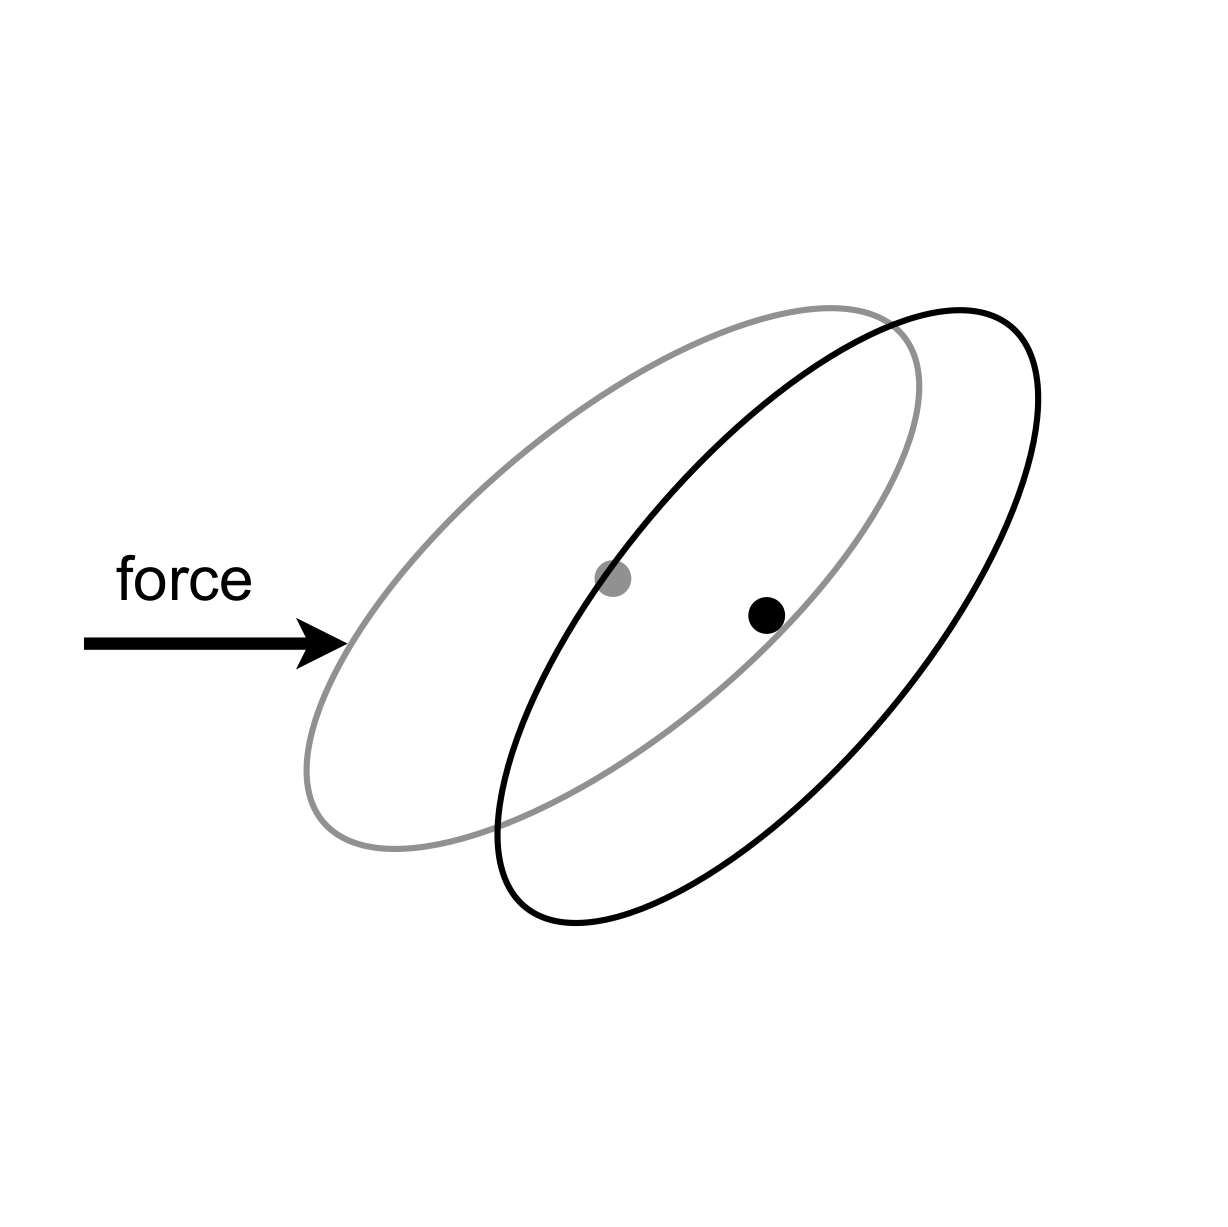
\includegraphics[width=1.80in]{left.png}
        \hspace{0.5in}
        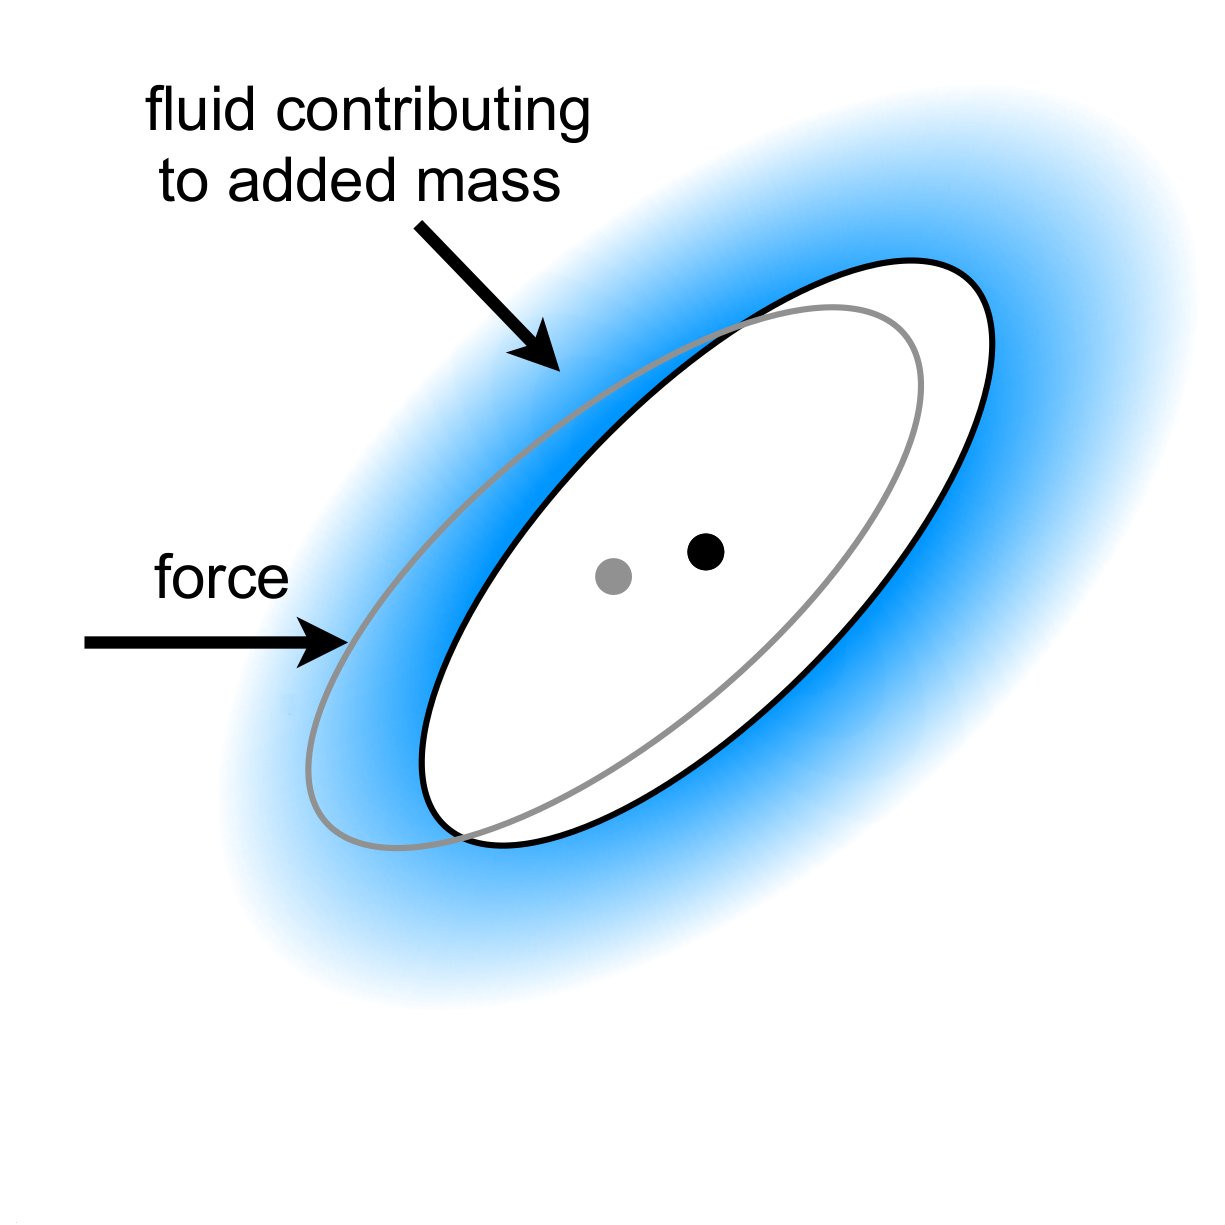
\includegraphics[width=1.80in]{right.png}
    \end{center}
\end{frame}

\begin{frame}
    \frametitle{The Immersed Boundary Method}
    \begin{figure}
        \centering
        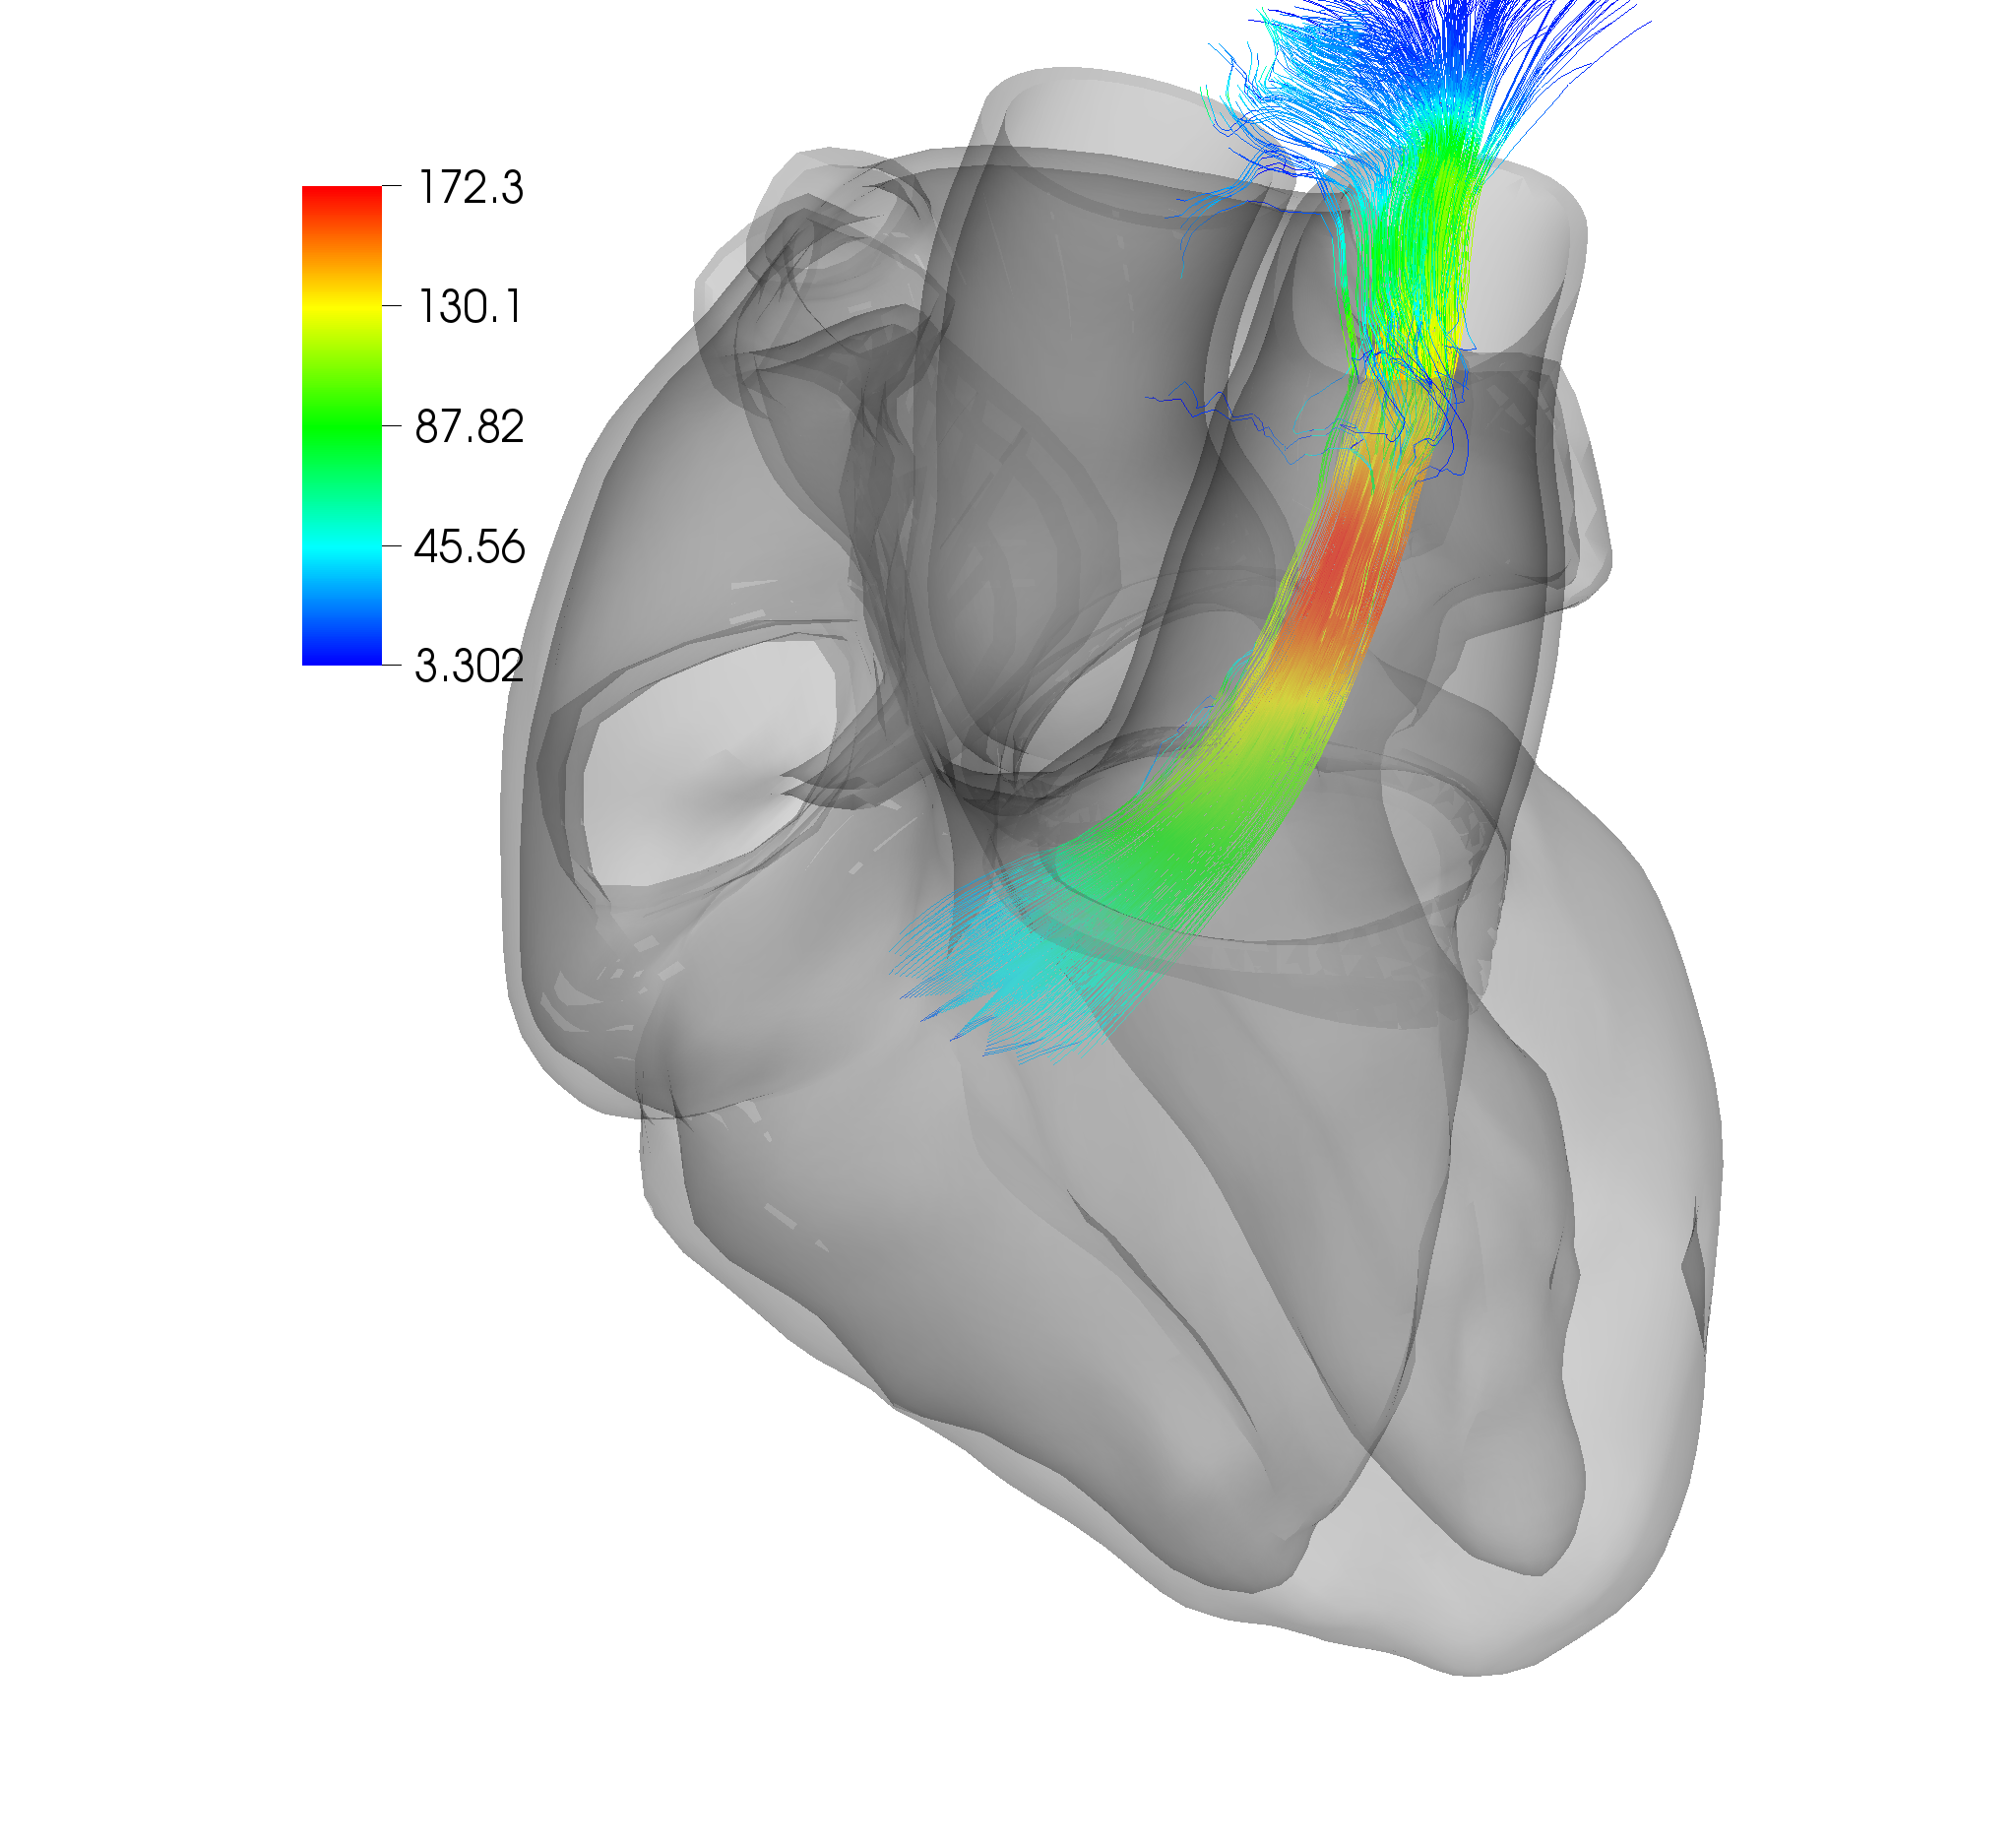
\includegraphics[width=2in]{vel_streamlines_RV.png}
    \end{figure}
    \begin{itemize}
        \item[$\blacksquare$] Solve for the fluid at all points (\emph{including
        inside the structure})
        \item[$\blacksquare$] Structure velocity given by fluid velocity
        \item[$\blacksquare$] Fluid force is given by the structure force
        density
        \item[$\blacksquare$] Coupling is done by regularized delta functions
        (\(\delta_h\))
    \end{itemize}
\end{frame}

\begin{frame}
    \frametitle{The Immersed Boundary Method}
    \begin{figure}
        \centering
        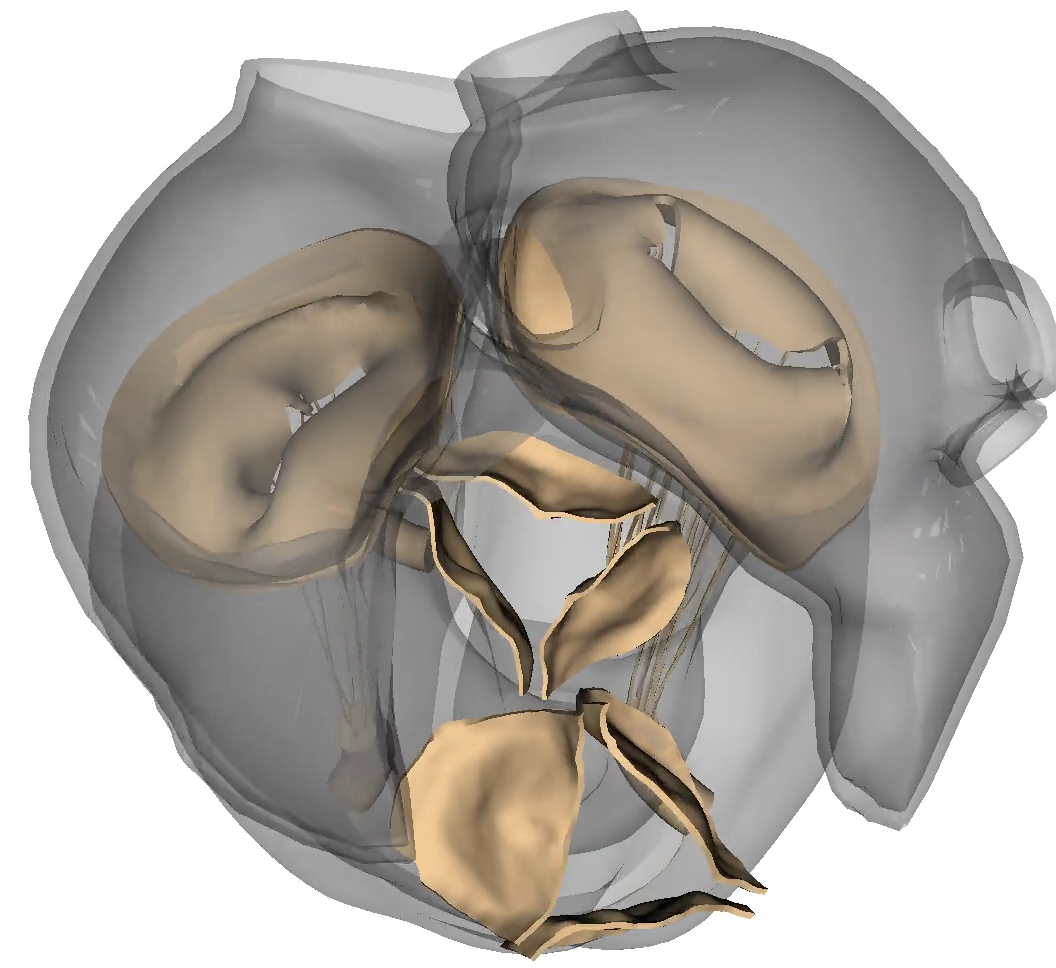
\includegraphics[width=1.5in]{mov3_Guccione0032.png}
    \end{figure}
    Advantages:
    \begin{itemize}
        \item[$\blacksquare$] Partitioned method
        \item[$\blacksquare$] Works well with really hard geometries
        \item[$\blacksquare$] Cartesian fluid domain
        \item[$\blacksquare$] No weird numerical instabilities
        \item[$\blacksquare$] coupling (velocity projection, force spreading)
        are adjoint operators: satisfy some conservation properties
    \end{itemize}
    Disadvantages:
    \begin{itemize}
        \item[$\blacksquare$] First order velocity convergence at
        fluid-structure boundaries (fix: \emph{Immersed Interface Method},
        Ebrahim Kolahdouz)
        \item[$\blacksquare$] Coupling occurs across a volume, not an interface
        (expensive)
    \end{itemize}
\end{frame}

\begin{frame}
    \frametitle{The Immersed Boundary Method}
    \begin{align*}
        \rho
        \left(
        \dfrac{\partial\mathbf{u}(\mathbf{x}, t)}{\partial t}
        + \mathbf{u}(\mathbf{x}, t) \cdot \nabla \mathbf{u}(\mathbf{x}, t)
        \right)
        &= -\nabla p(\mathbf{x}, t)
        + \mu \Delta \mathbf{u} (\mathbf{x}, t)
        + \mathbf{f}(\mathbf{x}, t),                                          \\
        \nabla \cdot \mathbf{u}(\mathbf{x}, t) &= 0,                          \\
        \dfrac{\partial \chi(\mathbf{X}, t)}{\partial t} &=
        \mathbf{u}(\chi(\mathbf{X}, t), t)
        = \int_\Omega \mathbf{u}(\mathbf{x}, t)
        \delta (\mathbf{x} - \chi(\mathbf{X}, t)) d\mathbf{x},                \\
        \mathbf{f}(\mathbf{x}, t) &=
        \int_{U} \mathbf{F}(\mathbf{X}, t)
        \delta(\mathbf{x} - \chi(\mathbf{X}, t)) d\mathbf{X},                 \\
        \int_U \mathbf{F}(\mathbf{X}, t) \cdot \phi(\mathbf{X}) d\mathbf{X}
        &= -\int_U\dfrac{\partial W}{\partial \mathbf{X}} : \nabla_{\mathbf{X}}
        \phi(\mathbf{X}) d\mathbf{X}, \forall \phi \in X^h(U)
    \end{align*}
    lower case variables are Eulerian, upper case are Lagrangian.
\end{frame}

\begin{frame}
    \frametitle{Fluid to Structure: Velocity Projection}
    \begin{figure}
        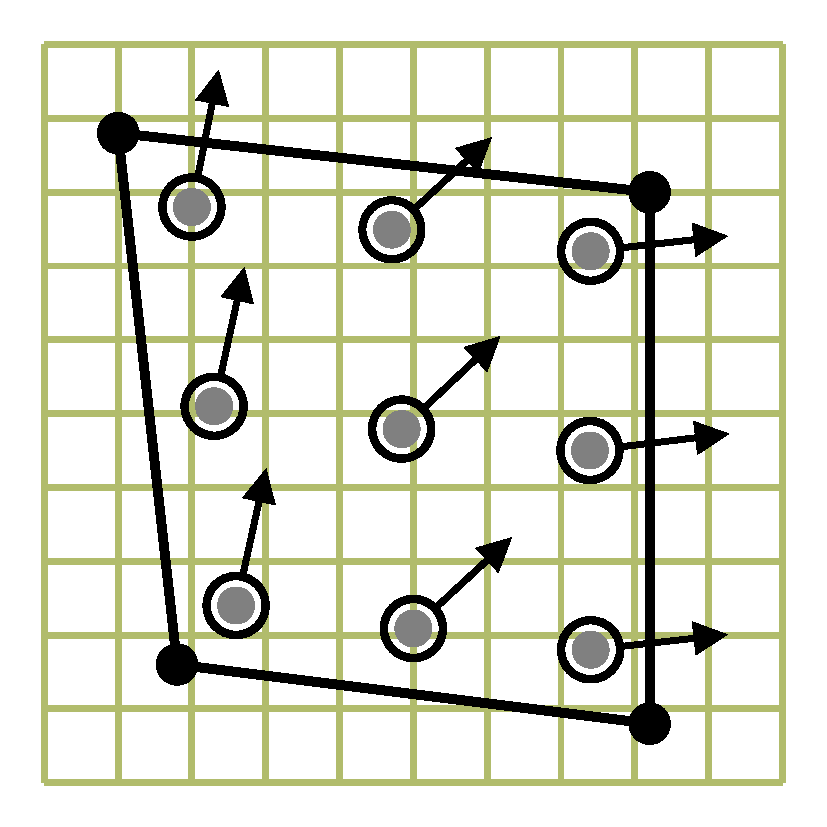
\includegraphics[width=2in]{gquad2d_4a-632.pdf}
    \end{figure}
    \begin{align*}
        \dfrac{\partial}{\partial t} \mathbf{\chi}(\mathbf{X}, t)
        &= \mathbf{U}(\mathbf{X}, t) \text{ where}                            \\
        \int_U \mathbf{U}(\mathbf{X}, t) \phi(\mathbf{X}) d\mathbf{X} &=
        \int_U \mathbf{V}(\mathbf{X}, t) \phi(\mathbf{X}) d\mathbf{X}, \forall
        \phi \in X^h(U)                                                       \\
        \mathbf{V}(\mathbf{X}, t) &= \sum_{i,j,k} \mathbf{u}_{i,j,k}
        \delta_h(\mathbf{x}_{i,j,k} - \mathbf{\chi}(\mathbf{X}, t))
        \Delta \mathbf{x}_{i,j,k}
    \end{align*}
\end{frame}

\begin{frame}
    \frametitle{Structure to Fluid: Force Spreading}
    \begin{figure}
        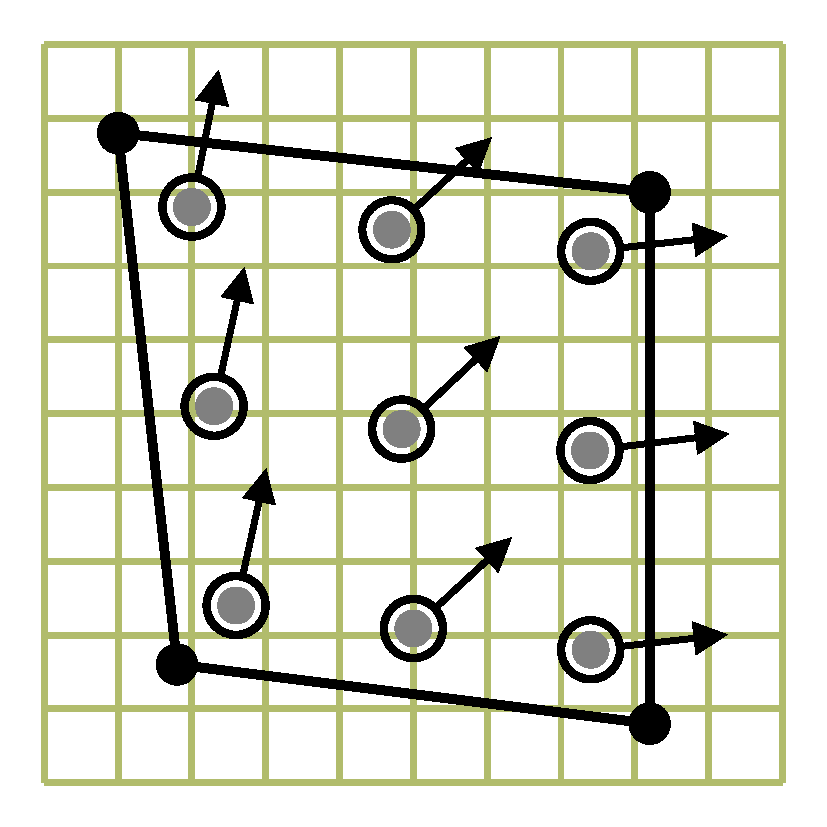
\includegraphics[width=2in]{gquad2d_4a-632.pdf}
    \end{figure}
    \begin{align*}
        \mathbf{f}(\mathbf{x}_{i,j,k}, t) &=
        \int_U \mathbf{F}(\mathbf{X}, t)
        \delta_h(\mathbf{x}_{i,j,k} - \mathbf{\chi}(\mathbf{X}, t))
        d \mathbf{X}                                                          \\
    \end{align*}
    Here \(-\mathbf{F}\) is the FE projection of the structural stress tensor (a
    force density). Comes from material models of heart tissue.
\end{frame}

\section{Where do we use PETSc?}
\begin{frame}
    \frametitle{Where do we use PETSc?}
    \begin{itemize}
        \item Common parallel backend (data, linear algebra)
        \item Students use it for very basic parallel synchronization (e.g.,
              rigid body, 6 degrees of freedom)
    \end{itemize}
\end{frame}

\begin{frame}
    \frametitle{Build System}
    \begin{itemize}
        \item Some interest in dependency management with BuildSystem
        \item Work in progress
    \end{itemize}
\end{frame}

\begin{frame}
    \frametitle{Fluid Solver}
    \begin{itemize}
        \item \texttt{KSP} solvers (duh!)
        \item Extensive use of \texttt{MatShell}
        \item sophisticated preconditioners: three operators, some do a single
              \(v\)-cycle
        \item Not SAMRAI's PETSc wrappers (we use an ancient version of SAMRAI
              that requires PETSc 2.3.3)
    \end{itemize}
\end{frame}

\begin{frame}
    \frametitle{Finite Elements}
    \begin{itemize}
        \item libMesh has good support for PETSc
        \item Use \texttt{Vec} via \texttt{libMesh::PetscVector<double>} (abuse
              its closing mechanism a lot)
        \item ``easy'' problem: \(L^2\) projection with conjugate gradient,
              block Jacobi preconditioner
    \end{itemize}
\end{frame}

\begin{frame}
    \frametitle{Fluid Structure Interaction}
    \begin{itemize}
        \item \emph{Challenge:} coordinate data between libMesh's and SAMRAI's
              parallel data distributions
        \item Currently assemble finite element contributions on \emph{Patches,
              not elements}, on the current processor
        \item Old approach: assemble load vector with \texttt{VecCache} (slow!)
        \item New approach: assemble into ghost entries, use
              \texttt{VecGhostUpdateBegin} and \texttt{VecGhostUpdateEnd}
              twice (sum then scatter)
        \item Future: generalize with \texttt{VecScatter}?
        \item Future: save communication patterns (currently hangs)
    \end{itemize}
\end{frame}
\end{document}
